\newsection{Beginner}

\underline{\textlg{\textbf{Questions are continued on the next page}}}
\newpage
\begin{enumerate}
%======================================================
\item \textbf{Time Difference}

%QUESTION SPECIFICS/IMAGES HERE
Given two times in HHMMSS format, print the time between them as HH:MM:SS. Assume both times are on the same day and the second is not earlier than the first.
%EXAMPLES HERE
\begin{consolethree}
Example 1:
Input: 091400 091415
Output: 00:00:15

Example 2:
Input: 095045 110510
Output: 01:14:25
\end{consolethree}
\newpage

%======================================================
\item \textbf{Print the calendar}

%QUESTION SPECIFICS/IMAGES HERE
Given a month, year, and weekday of the first day, print that month's calendar. Weekdays are numbered 0 (Sunday) through 6 (Saturday). Account for leap years.
%EXAMPLES HERE
\begin{consolethree}
Example 1:
Input: month = 3, year = 2008, firstWeekday = 6

Output:
March 2008
Su  Mo  Tu  We  Th  Fr  Sa
                         1
 2   3   4   5   6   7   8
 9  10  11  12  13  14  15
16  17  18  19  20  21  22
23  24  25  26  27  28  29
30  31
\end{consolethree}
\newpage


%======================================================
\item \textbf{Check a Map Position}

%QUESTION SPECIFICS/IMAGES HERE
Given a row $r$ and column $c$, print 1 if the position is open and 0 if it is blocked or outside the map.

Rows are numbered 0–7 and columns 0–9.

The blocked areas are:
	Rows 1–2, columns 2–8.
	Rows 5–6, columns 4–7.


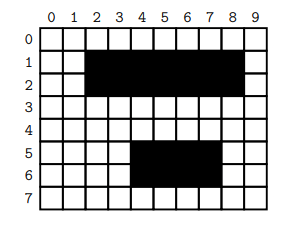
\includegraphics[scale=0.45]{images/rowcol.png}


%EXAMPLES HERE
\begin{consolethree}
Example 1:
Input: r = 0, c = 0
Output: 1

Example 2:
Input: r = 1, c = 4
Output: 0

\end{consolethree}
\newpage


%======================================================
\item \textbf{Print a V}

%QUESTION SPECIFICS/IMAGES HERE
Given a positive integer n, print a V made of stars with n rows.

%EXAMPLES HERE
\begin{consolethree}
Example 1:
Input: 1
Output:
*

Example 2:
Input: 2
Output:
* *
 *
  
Example 3:
Input: 4
Output:
*   *
 * *
  *
\end{consolethree}
\newpage


%======================================================
\item \textbf{Magic Squares}

%QUESTION SPECIFICS/IMAGES HERE
Print all 3-by-3 arrangements of the digits 1–9 where every row, column, and both diagonals add to 15. Use each digit exactly once. There is no input.

Your program should find all 8 arrangements. Rotations and reflections count as different arrangements.

The first two magic squares are shown below:
%EXAMPLES HERE
\begin{consolethree}
Example 1:
2 7 6
9 5 1
4 3 8

4 9 2
3 5 7
8 1 6
\end{consolethree}
\newpage


%======================================================
\item \textbf{Prime Search and Factorization}

%QUESTION SPECIFICS/IMAGES HERE
Compute and store the first 100,000 primes in an array. Print the first 5 and last 5.

Then repeatedly read a number x and an option:
Option 0: Use binary search to check whether x is prime. If it is, print its array index, starting at 0.
Option 1: Print x as a product of prime factors.
Stop when x is -1.

Assume x is at least 2 and any prime needed is in your array. For option 0, x will not exceed the largest stored prime.

%EXAMPLES HERE
\begin{consolethree}
Example 1:
Input: x = 13, option = 0
Output: Prime, index 5

Example 2:
Input: x = 12, option = 0
Output: Not prime

Example 3:
Input x = 60, option = 1
Output: 2 * 2 * 3 * 5
\end{consolethree}
\newpage



%======================================================
\item \textbf{Sums of Two Cubes}

%QUESTION SPECIFICS/IMAGES HERE
Given a positive integer n, print all positive integers x, y, and z where x³ + y³ = z and z is at most n. Print each solution as x y z, ordered by z and then x. Include reversed pairs.

%EXAMPLES HERE
\begin{consolethree}
Example 1:
Input: 16
Output:
1 1 2
1 2 9
2 1 9
2 2 16

Explanation: 1 2 9 means |\texttt{$1^3$ + $2^3$}| = 9.
\end{consolethree}
\newpage



%======================================================
\item \textbf{Add Fractions}

%QUESTION SPECIFICS/IMAGES HERE
Given four integers a, b, c, and d, where a / b and c / d are viewed as fractions. Simplify the result. If it is a whole number, print it without a denominator. Assume denominators are positive.

%EXAMPLES HERE
\begin{consolethree}
Example 1:
Input: 1 6 1 3
Output: 1/2

Example 2:
Input: 3 4 5 4
Output: 2
\end{consolethree}
\newpage



%======================================================
\item \textbf{Add Digits}

%QUESTION SPECIFICS/IMAGES HERE
Given a nonnegative integer, repeatedly add its digits until only one digit remains.

%EXAMPLES HERE
\begin{consolethree}
Example 1:
Input: 38
Output: 2
Explanation: 3 + 8 = 11, then 1 + 1 = 2.

Example 2:
Input: 0
Output: 0
\end{consolethree}
\newpage



%======================================================
\item \textbf{Plus One}
%QUESTION SPECIFICS/IMAGES HERE

Given an array representing the digits of a nonnegative integer, add 1 and return the resulting digits. Work directly with the array rather than converting the entire number to an integer.

%EXAMPLES HERE
\begin{consolethree}
Example 1:
Input: [1, 2, 3]
Output: [1, 2, 4]

Example 2:
Input: [9, 9]
Output: [1, 0, 0]
\end{consolethree}
\newpage



%======================================================
\item \textbf{Merge Sorted Arrays}

%QUESTION SPECIFICS/IMAGES HERE
Given two sorted arrays, merge them into nums1 in sorted order. The first m elements of nums1 are actual values; its remaining n spaces are placeholders. nums2 contains n actual values.

%EXAMPLES HERE
\begin{consolethree}
Example 1: nums1 = [1, 2, 3, 0, 0, 0],
		   nums2 = [2, 5, 6],
		   n = 3,
		   m = 3
		   
Output: nums1 = [1, 2, 2, 3, 5, 6]

The placeholder zeros are ignored. Keep duplicate values.
\end{consolethree}
\newpage



%======================================================
\item \textbf{Search Insert Position}

%QUESTION SPECIFICS/IMAGES HERE
Given a sorted array of distinct integers and a target, return the target's index. If it is missing, return the index where it would be inserted. Indices start at 0. Use binary search.

%EXAMPLES HERE
\begin{consolethree}
Example 1: [1, 3, 5, 6], target = 5
Output:    2

Example 2: [1, 3, 5, 6], target = 2
Output:    1

Example 3: [1, 3, 5, 6], target = 7
Output:    4
\end{consolethree}
\newpage



%======================================================
\item \textbf{Zigzag Conversion}

%QUESTION SPECIFICS/IMAGES HERE
Given a string and a number of rows, place characters into rows by moving down, then up, repeatedly. Return the characters read one row at a time from top to bottom.
For 3 rows, characters go into rows 0, 1, 2, 1, 0, 1, 2, and so on.

If there is only one row, return the original string.
%EXAMPLES HERE
\begin{consolethree}
Example 1: "PAYPALISHIRING", rows = 3
Output:    "PAHNAPLSIIGYIR"
Explanation:
Row 0: PAHN
Row 1: APLSIIG
Row 2: YIR
\end{consolethree}
\newpage



%======================================================
\item \textbf{Ugly Number}

%QUESTION SPECIFICS/IMAGES HERE
Given an integer, return true if it is positive and its only prime factors are 2, 3, and 5. Otherwise, return false. The number 1 also counts as ugly.


%EXAMPLES HERE
\begin{consolethree}
Example 1: 6
Output:    true
Explanation: 6 = 2 * 3.

Example 2: 14
Output:    false
Explanation: 14 has a prime factor of 7.
\end{consolethree}
\newpage



%======================================================
\item \textbf{Two Sum}

%QUESTION SPECIFICS/IMAGES HERE
Given an integer array and a target, return the indices of two elements that add to the target. Indices start at 0. There is exactly one valid pair, and you cannot use the same element twice.

%EXAMPLES HERE
\begin{consolethree}
Example 1: [2, 7, 11, 15], target = 9
Output:    [0, 1]

Example 2: [3, 3], target = 6
Output:    [0, 1]
\end{consolethree}
\newpage



%======================================================
\item \textbf{Integer Square Root}

%QUESTION SPECIFICS/IMAGES HERE
Given a nonnegative integer x, return its square root rounded down. Do not use built-in square-root or exponent functions.

%EXAMPLES HERE
\begin{consolethree}
Example 1: 4
Output:    2

Example 2: 8
Output:    2

Explanation: 2 * 2 is at most 8, but 3 * 3 is greater than 8.
\end{consolethree}
\newpage



%======================================================
\item \textbf{Longest Common Prefix}

%QUESTION SPECIFICS/IMAGES HERE
Given an array of strings, return the longest beginning shared by every string. Return "" if there is no shared beginning.

%EXAMPLES HERE
\begin{consolethree}
Example 1: ["flower", "flow", "flight"]
Output:    "fl"

Example 2: ["dog", "racecar", "car"]
Output:    ""
\end{consolethree}
\newpage



%======================================================
\item \textbf{Rotated Digits}

%QUESTION SPECIFICS/IMAGES HERE
Given a positive integer n, count the numbers from 1 through n that become different valid numbers when every digit is replaced using these rules:
0, 1, and 8 stay unchanged.
2 becomes 5, and 5 becomes 2.
6 becomes 9, and 9 becomes 6.
3, 4, and 7 make the number invalid.
Keep the digits in the same positions. Count a number only if all digits are valid and at least one changes.

%EXAMPLES HERE
\begin{consolethree}
Example 1: 10
Output:    4
Explanation: The qualifying numbers are 2, 5, 6, and 9.
\end{consolethree}
\newpage

\end{enumerate}
